\documentclass[12pt]{article}
\usepackage[utf8]{inputenc}

\usepackage{lmodern}

\usepackage{enumitem}
\usepackage[margin=2cm]{geometry}

\usepackage{amsmath, amsfonts, amssymb}
\usepackage{graphicx}
%\usepackage{subfigure}
\usepackage{tikz}
\usepackage{pgfplots}
\usepackage{multicol}

\usepackage{comment}
\usepackage{url}
\usepackage{calc}
\usepackage{subcaption}
\usepackage[indent=0pt]{parskip}
\usepackage{animate}

\usepackage{array}
\usepackage{blkarray,booktabs, bigstrut}
\usepackage{bigints}

\pgfplotsset{compat=1.16}

% MATH commands
\newcommand{\ga}{\left\langle}
\newcommand{\da}{\right\rangle}
\newcommand{\oa}{\left\lbrace}
\newcommand{\fa}{\right\rbrace}
\newcommand{\oc}{\left[}
\newcommand{\fc}{\right]}
\newcommand{\op}{\left(}
\newcommand{\fp}{\right)}

\newcommand{\bi}{\mathbf{i}}
\newcommand{\bj}{\mathbf{j}}
\newcommand{\bk}{\mathbf{k}}
\newcommand{\bF}{\mathbf{F}}

\newcommand{\mR}{\mathbb{R}}

\newcommand{\ra}{\rightarrow}
\newcommand{\Ra}{\Rightarrow}

\newcommand{\sech}{\mathrm{sech}\,}
\newcommand{\csch}{\mathrm{csch}\,}
\newcommand{\curl}{\mathrm{curl}\,}
\newcommand{\dive}{\mathrm{div}\,}

\newcommand{\ve}{\varepsilon}
\newcommand{\spc}{\vspace*{0.5cm}}

\DeclareMathOperator{\Ran}{Ran}
\DeclareMathOperator{\Dom}{Dom}

\newcommand{\exo}[1]{\noindent\textcolor{red}{\fbox{\textbf{Problem {#1}}}\hrulefill}\\}
\newcommand{\qu}[4]{\noindent\textcolor{#4}{\fbox{\textbf{Section {#1} | Problem {#2}}} \hrulefill{{\fbox{\textbf{{#3} Points}}}}\\}}

\newcommand{\semester}{Spring 2023}

\newcommand{\CVup}{%
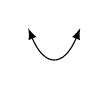
\begin{tikzpicture}
\draw[black, <->, >=latex] (-0.33, 0.5) .. controls (-0.125, 0) and (0.125, 0) .. (0.33, 0.5);
\end{tikzpicture}}

\newcommand{\CVupInc}{%
\begin{tikzpicture}
\draw[black, ->, >=latex] (0,0) .. controls (0.2, 0) and (0.4, 0.2) .. (0.5, 0.5);
\end{tikzpicture}}

\newcommand{\CVupDec}{%
\begin{tikzpicture}[rotate=270]
\draw[black, ->, >=latex] (0,0) .. controls (0.2, 0) and (0.4, 0.2) .. (0.5, 0.5);
\end{tikzpicture}}

\newcommand{\CVdown}{%
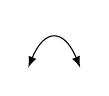
\begin{tikzpicture}
\draw[black, <->, >=latex] (-0.33, -0.5) .. controls (-0.125, 0) and (0.125, 0) .. (0.33, -0.5);
\end{tikzpicture}}

\newcommand{\CVdownInc}{%
\begin{tikzpicture}
\draw[black, ->, >=latex] (-0.5, -0.5) .. controls (-0.5, -0.3) and (-0.5, -0.1) .. (0,0);
\end{tikzpicture}}

\newcommand{\CVdownDec}{%
\begin{tikzpicture}[rotate=-90]
\draw[black, ->, >=latex] (-0.5, -0.5) .. controls (-0.5, -0.3) and (-0.5, -0.1) .. (0,0);
\end{tikzpicture}}

\begin{document}
	\noindent \hrulefill \\
	MATH-241 \hfill Pierre-Olivier Paris{\'e}\\
	Solutions Section 1-4 \hfill \semester \\\vspace*{-1cm}
	
	\noindent\hrulefill
	
	\spc
	
	\exo{4}
	
	\begin{enumerate}
	\item[(a)] Let $y = \cos \pi x$. 
		\begin{enumerate}
		\item[(ii)] The slope of $PQ$ is
			\begin{align*}
			m_{PQ} = \frac{\cos (0.5\pi) - \cos (0.4\pi)}{0.5 - 0.4} = \frac{-\cos (0.4 \pi )}{0.1} = -3.090170 .
			\end{align*}
		\item[(iii)] The slope of $PQ$ is
			\begin{align*}
			m_{PQ} = \frac{\cos (0.5\pi ) - \cos (0.49 \pi )}{0.5 - 0.49} = - \frac{\cos (0.49 \pi )}{0.01} = -3.141076 .
			\end{align*}
		\item[(iv)] The slope of $PQ$ is
			\begin{align*}
			m_{PQ} = \frac{\cos (0.5 \pi ) - \cos (0.499 \pi )}{0.5 - 0.499} = - \frac{\cos (0.499 \pi )}{0.001} = -3.141586 .
			\end{align*}
		\item[(vi)] The slope of $PQ$ is
			\begin{align*}
			m_{PQ} = \frac{\cos (0.5 \pi ) - \cos (0.6 \pi)}{0.5 - 0.6} = \frac{\cos (0.6 \pi)}{0.1} = -3.090170 .
			\end{align*}
		\item[(vii)] The slope of $PQ$ is
			\begin{align*}
			m_{PQ} = \frac{\cos (0.5 \pi ) - \cos (0.51 \pi )}{0.5 - 0.51} = \frac{\cos (0.51 \pi )}{0.01} = -3.141076 .
			\end{align*}
		\item[(viii)] The slope of $PQ$ is
			\begin{align*}
			m_{PQ} = \frac{\cos (0.5 \pi ) - \cos (0.501 \pi )}{0.5 - 0.501} = \frac{\cos (0.501 \pi )}{0.001} = -3.141586 .
			\end{align*}
		\end{enumerate}
	\item[(b)] The slope would be $-\pi$.
	\item[(c)] The equation of a line with slope $-\pi$ is $y - y_0 = -\pi (x - x_0 )$ where the line passes through the point $(x_0 , y_0 )$. Therefore, since $(0.5, 0)$ is on the line, we get
		\begin{align*}
		y = -\pi (x - 0.5) = -\pi x + \pi/2 .
		\end{align*}
	\item[(d)] Plot using Desmos.
	\end{enumerate}
	
	\spc
	
	\exo{8}
	\begin{enumerate}[label=(\alph*)]
	\item
	\begin{enumerate}[label=(\roman*)]
	\item $v_{ave} = \frac{s(2) - s(1)}{2 - 1} = 3 - (-3) = 6 \, \text{cm/s}$.
	\item $v_{ave} = \frac{s(1.1) - s(1)}{1.1 - 1} \approx -4.7120\,\text{cm/s}$.
	\item $v_{ave} = \frac{s(1.01) - s(1)}{1.01 - 1} \approx -6.1341 \,\text{cm/s}$.
	\item $v_{ave} = \frac{s(1.001) - s(1)}{1.001 -1} \approx -6.2683 \,\text{cm/s}$.
	\end{enumerate}
	\item We first give an estimation using a point on the left side of $1$, say $0.999$. We get $v_{ave} \approx -6.2746 \text{cm/s}$. So we estimate the instantaneous velocity as
		\begin{align*}
		v \approx \frac{-6.2683 + (-6.2746)}{2} = -6.2714\,\text{cm/s} .
		\end{align*}
	\end{enumerate}
	
\end{document}